\documentclass[12pt]{article}
\usepackage[margin=2.5cm]{geometry}
\usepackage{enumerate}
\usepackage{amsfonts}
\usepackage{amsmath}
\usepackage{fancyhdr}
\usepackage{amsmath}
\usepackage{amssymb}
\usepackage{amsthm}
\usepackage{mdframed}
\usepackage{graphicx}
\usepackage{subcaption}
\usepackage{adjustbox}
\usepackage{listings}
\usepackage{xcolor}
\usepackage{booktabs}
\usepackage[utf]{kotex}

\definecolor{codegreen}{rgb}{0,0.6,0}
\definecolor{codegray}{rgb}{0.5,0.5,0.5}
\definecolor{codepurple}{rgb}{0.58,0,0.82}
\definecolor{backcolour}{rgb}{0.95,0.95,0.92}

\lstdefinestyle{mystyle}{
    backgroundcolor=\color{backcolour},
    commentstyle=\color{codegreen},
    keywordstyle=\color{magenta},
    numberstyle=\tiny\color{codegray},
    stringstyle=\color{codepurple},
    basicstyle=\ttfamily\footnotesize,
    breakatwhitespace=false,
    breaklines=true,
    captionpos=b,
    keepspaces=true,
    numbers=left,
    numbersep=5pt,
    showspaces=false,
    showstringspaces=false,
    showtabs=false,
    tabsize=1
}

\lstset{style=mystyle}

\pagestyle{fancy}
\renewcommand{\headrulewidth}{0.4pt}
\lhead{Hyungmo Gu}
\rhead{CSC209 Week 8 Notes}

\begin{document}
\title{CSC209 Week 8 Notes}
\author{Hyungmo Gu}
\maketitle

\section*{Processes 1 of 8}

\bigskip

\begin{itemize}
    \item Process Models
    \begin{itemize}
        \item Program
        \begin{itemize}
            \item The executable instructions of a program
            \item Source code
            \item Compiled machine code

            \begin{center}
            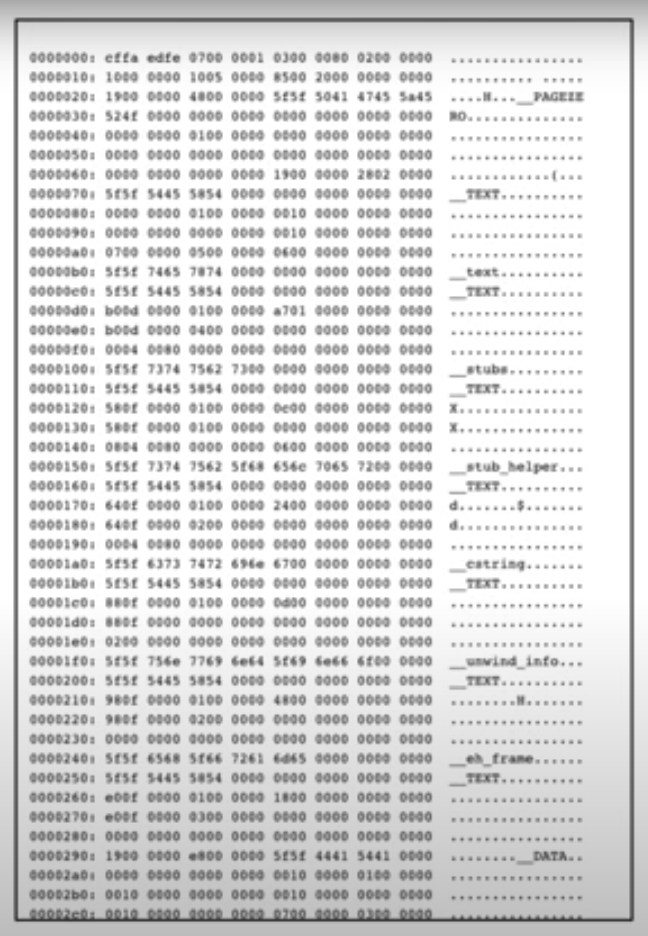
\includegraphics[width=0.5\linewidth]{images/week_8_notes_1_1.png}
            \end{center}

        \end{itemize}
        \item Process
        \begin{itemize}
            \item Running instance of program
        \end{itemize}

        \item Process Control Block (PCB)
        \begin{itemize}
            \item is a data structure used by computer operating system to
            store all information about process.
            \item Code, Global, Heap and Stack together are called the \textbf{State of Program}
            \begin{center}
            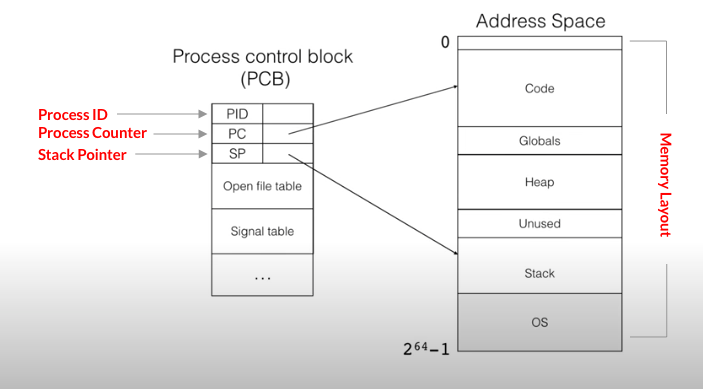
\includegraphics[width=\linewidth]{images/week_8_notes_1_3.png}
            \end{center}

            \begin{itemize}
                \item \textbf{Code:} is program code
                \item \textbf{Stack:} tells which function is being executed, and hold
                values of local variables
                \item \textbf{Heap and Globals:} holds current value for other variables in the program
            \end{itemize}

            \item is also known as \textbf{process descriptor}
            \begin{enumerate}[1.]
                \item When a process is created (initialized or installed), the
                operating system creates a corresponding process control block.
                \item Information in a process lbock is updated during the
                transition of process states
                \item When the process terminates, its PCB is returned to the pool
                from which new PCBs are drawn
                \item Each process has a single PCB
            \end{enumerate}

        \end{itemize}

        \item Top

        \begin{itemize}
            \item is a basic unix command useful for observing current state of
            Unix System.

            \begin{center}
            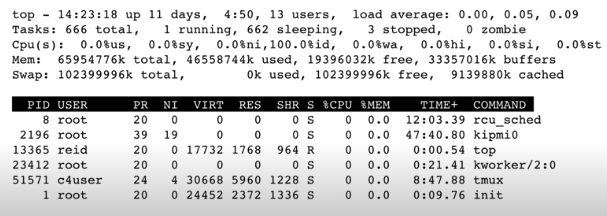
\includegraphics[width=\linewidth]{images/week_8_notes_1_2.png}
            \end{center}
        \end{itemize}

        \item Three-state Process Management Model
        \begin{center}
        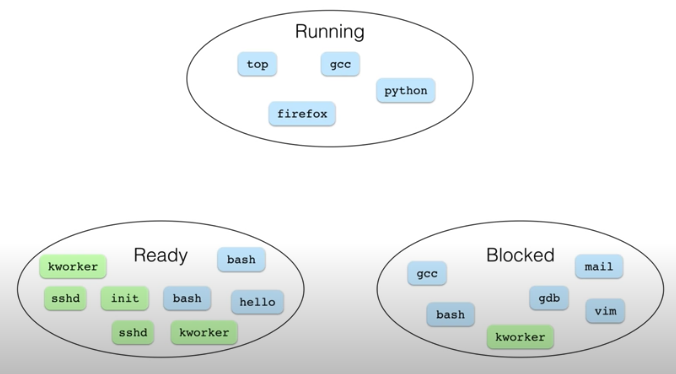
\includegraphics[width=0.8\linewidth]{images/week_8_notes_1_4.png}
        \end{center}

        \begin{itemize}
            \item Works with PCB
            \item Works simultaneously on multiple processors
            \item A program is in either one of three states:
            \begin{itemize}
                \item \textbf{Running:} The process that is currently being executed
                \item \textbf{Ready:} A process that is queuing and prepare to execute when given the opportunity
                \item \textbf{Blocked:} A process that cannot execute until some event occurs,
                i.e. waking up from sleep
            \end{itemize}
        \end{itemize}
    \end{itemize}
\end{itemize}

\bigskip

\section*{Processes 2 of 8}

\bigskip

\begin{itemize}
    \item Creating Processes with Fork
    \begin{itemize}
        \item fork()
        \begin{itemize}
            \item is a part of \textit{unistd.h} library.
            \item creates a new process, which is called child process, which runs
            \item starts executing after fork() is called
        \end{itemize}

        \bigskip

    \begin{lstlisting}[language=c,caption={process\_example\_1.c}]
    #include <stdio.h>
    #include <unistd.h> // <- fork imported here

    int main() {
        int i;
        pid_t result;

        i = 5;
        printf("%d\n", i);

        result = fork(); // <- Here is the fork :)

        if (result > 0) {
            i = i + 2;
        } else if (result == 0) {
            i = i - 2;
        } else {
            perror("fork");
        }

        printf("%d\n", i);
        return 0;
    }
    \end{lstlisting}

    \end{itemize}
\end{itemize}

\bigskip

\section*{Processes 3 of 8}

\bigskip

\begin{itemize}
    \item Process Relationship and Termination (Part 1)
    \begin{itemize}
        \item Parent and child processes don't occur in order
        \item Child processes not in order since they are running concurrently
        \item Key Queston: How to make the parent to wait before child finishes?
    \begin{lstlisting}[language=c]
    // Output of process_example_2.c
    // Run by typing gcc -Wall process_example_2.c

    [20480] Original process (my parent is 15738)
    [20481] Child 0 0
    [20481] Child 0 1
    [20482] Child 1 0 //<- notice 1 starts before 0 ends
    [20481] Child 0 2
    [20482] Child 1 1
    [20481] Child 0 3
    [20483] Child 2 0
    [20482] Child 1 2
    [20481] Child 0 4
    [20480] Parent about to terminate // <- notice parent ends before children
    [20482] Child 1 3
    [20483] Child 2 1
    [20484] Child 3 0 //<- notice 3 starts before 1 and 2 ends
    [20482] Child 1 4
    [20483] Child 2 2
    [20484] Child 3 1
    [20485] Child 4 0
    [20483] Child 2 3
    [20484] Child 3 2
    [20483] Child 2 4
    [20485] Child 4 1
    [20484] Child 3 3
    [20485] Child 4 2
    [20484] Child 3 4
    [20485] Child 4 3
    [20485] Child 4 4
    \end{lstlisting}
    \end{itemize}
\end{itemize}

\bigskip

\section*{Processes 4 of 8}

\bigskip

\begin{itemize}
    \item wait
    \begin{itemize}
        \item \textbf{Syntax:} pid\_t\ wait(int *wstatus)
        \item Is a part of \textit{sys/wait.h} library.
        \item Blocks the calling process until one of its child processes exists
        or a signal is received.
        \item Parent continues its execution after wait call
    \end{itemize}
    \item WIFEXITED
    \begin{itemize}
        \item \textbf{Syntax:} int WIFEXITED (int status)
        \item Checks if child exited normally
        \item Returns non-zero if true
    \end{itemize}
    \item WIFEXITSTATUS(status)
    \begin{itemize}
        \item \textbf{Syntax:} int WIFEXITSTATUS (int status)
        \item Returns code when child exits
    \end{itemize}
    \item WTERMSIG
    \begin{itemize}
        \item \textbf{Syntax:} int WTERMSIG (int status)
        \item Returns non-zero value if the child process terminated due to a signal,
        i.e. abort()
    \end{itemize}

    \begin{lstlisting}[language=c,caption={process\_example\_3.c}]
    #include <stdio.h>
    #include <unistd.h>
    #include <stdlib.h>
    #include <signal.h>

    int main() {
        ...

        for(i = 0; i < 5; i++) {
            pid_t pid;
            int status;
            if ((pid = wait(&status)) == -1) { // <- wait called here
                perror("wait");
            } else {
                if (WIFEXITED(status)) { // <- processes ended normally
                    printf("Child %d terminated with %d\n", pid, WEXITSTATUS(status));
                } else if (WIFSIGNALED(status)) { // <- child exited due to signal
                    printf("Child %d terminated with signal %d\n", pid, WTERMSIG(status));
                } else {
                    printf("Shouldn't get here");
                }
            }
        }
        printf("[%d] Parent about to terminate\n", getpid());
        return 0;
    }
    \end{lstlisting}
\end{itemize}

\bigskip

\section*{Processes 6 of 8}

\bigskip

\begin{itemize}
    \item Running Different Programs
    \begin{itemize}
        \item execl
        \begin{itemize}
            \item \textbf{Syntax:} int execl(const char *filepath, [const char *arg1, const char *arg2], NULL)
            \item is a part of \textit{unistd.h} library
            \item Requires \textit{NULL} as final arguement
            \item Code doesn't return to main if excel is successful
            \item Code returns to main if excel is unsuccessful
        \end{itemize}
    \end{itemize}

    \begin{lstlisting}[language=c,caption={process\_example\_4.c}]
    #include <stdio.h>
    #include <unistd.h>

    int main() {
        printf("About to call excel. My PID is %d\n", getpid());
        execl("./hello.out", NULL); // <- searches for .out
        perror("exec");
        return 1;
    }
    \end{lstlisting}

\end{itemize}


\end{document}